\documentclass{beamer}
%\usecolortheme{dove} %Make title black
\usepackage{graphicx} % Allows including images
\usepackage{booktabs} % Allows the use of \toprule, \midrule and \bottomrule in tables
%\usepackage{siunitx}  %Use SI unit formatting
%\sisetup{range-phrase=--}
%Bold command
%\newcommand\SEC[1]{\textbf{\uppercase{#1}}}
\usepackage{pifont}% http://ctan.org/pkg/pifont
\newcommand{\cmark}{\ding{51}}%
\newcommand{\xmark}{\ding{55}}%
%\usepackage{siunitx}  %Use SI unit formatting
%For drawing beam line
\include{tikz}
\usetikzlibrary{shapes.misc}
\usetikzlibrary{shapes,arrows,decorations.markings,shadows,positioning}
%Adjust width of slide
\newcommand\Wider[2][3em]{%
	\makebox[\linewidth][c]{%
		\begin{minipage}{\dimexpr\textwidth+#1\relax}
			\raggedright#2
		\end{minipage}%
	}%
}

\include{header}
\usebackgroundtemplate{
\includegraphics[width=\paperwidth]{NormalANLMaroon.pdf}}
\title[PSI Talk]{Photoinjector simulations for the Argonne Wakefield Accelerator facility}
\author[Speaker]{Nicole Neveu}
\subtitle{}
\institute[ANL/IIT]{Argonne National Laboratory\\Illinois Institute of Technology}
\date{\today}

\logo{%
	\makebox[0.95\paperwidth]{%
		%\includegraphics[width=3cm,keepaspectratio]{IIT_logo}%
		\hfill%
		\includegraphics[width=2.5cm,keepaspectratio]{IIT_logo_blk}%
	}%
}

\setbeamertemplate{navigation symbols}{}


%------------------------------------------------------
\begin{document}
\setbeamertemplate{footline}[page number]{}
{
	\usebackgroundtemplate{
\includegraphics[width=\paperwidth]{TitleANLMaroon}}
	\logo{%
		\makebox[0.95\paperwidth]{%
			\includegraphics[width=3cm,keepaspectratio]{IIT_logo}%
			\hfill%
			%\includegraphics[width=3cm,keepaspectratio]{IIT_logo_blk}%
		}%
	}
	\frame{\titlepage}
}

%\setbeamertemplate{footline}[]{}	
	
% FRAME: overview
\begin{frame}
  \frametitle{Outline}
  \tableofcontents
\end{frame}
% ========================================
% main slides come here
% ========================================
\section{Facility Introduction}
%\begin{frame}
%  \frametitle{Before we start ...}
%\end{frame}

\begin{frame}[plain]
\frametitle{AWA Facility}
\Wider[4em]{
  \setlength{\leftmargin}{0.1cm}
  \begin{itemize}
    \item{Two photocathode guns and accompanying linacs}
    \begin{itemize}
      \item{\underline{\textbf{Drive Line}}: $Cs_2Te$ cathode, 6 linac cavities}
      \begin{itemize}
        \item{Charge 0.1-100nC}
        \item{Energy up to 70 MeV}
        
      \end{itemize}
      \item{\underline{\textbf{Witness Line}}: $Mg$ cathode, 1 linac cavity}
      \begin{itemize}
        \item{Charge 0.1-10nC}
        \item{Energy up to 15 MeV}
      \end{itemize}
    \end{itemize}
\end{itemize}
\centering
 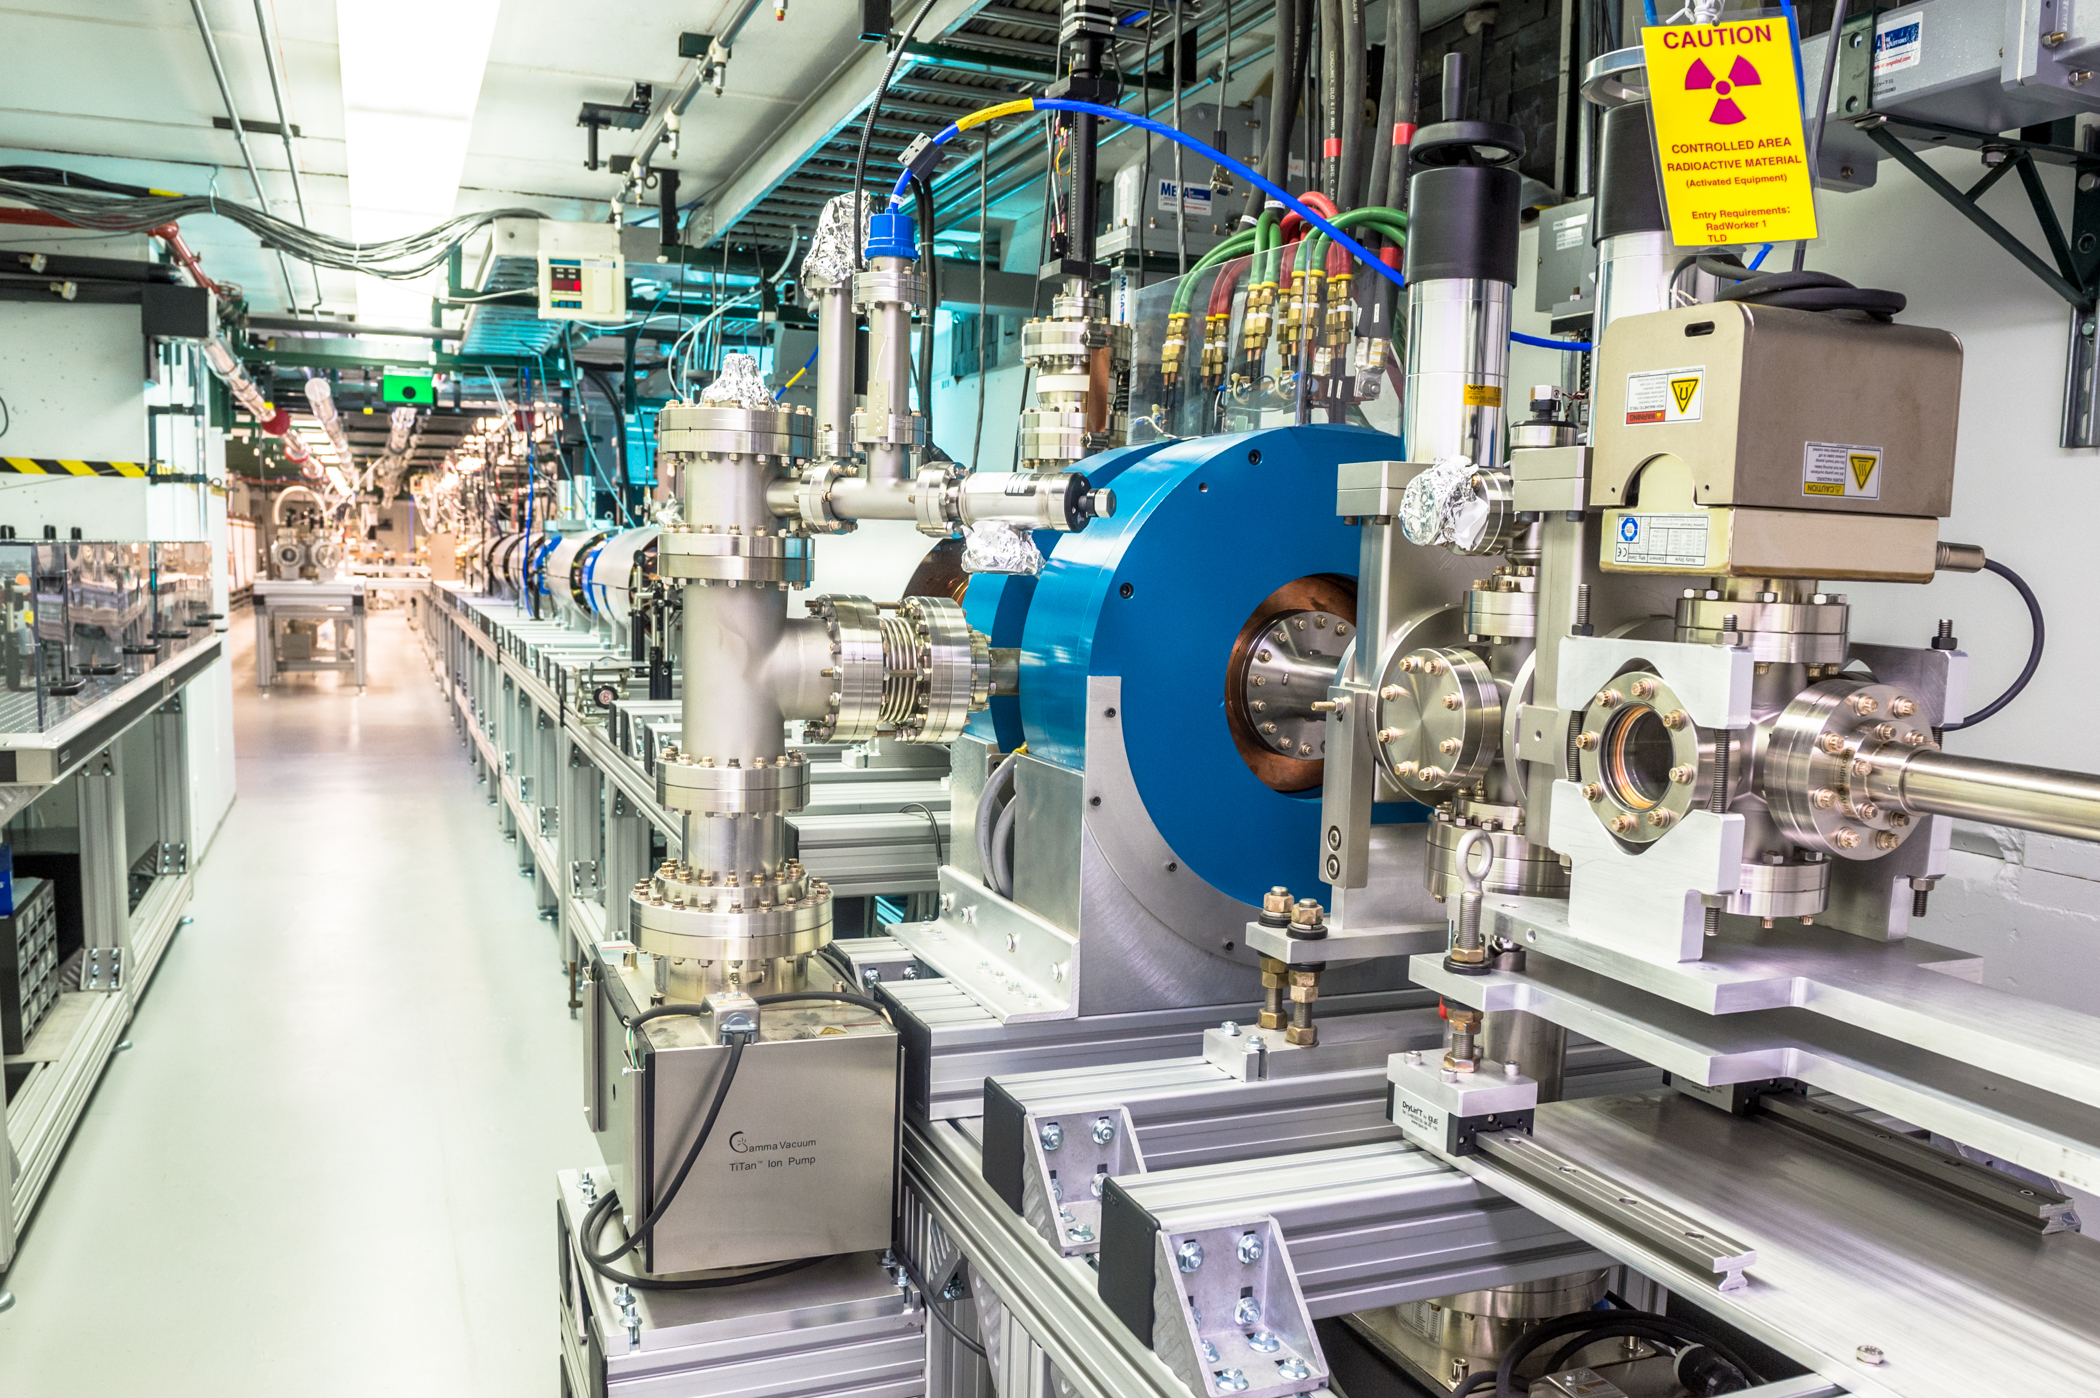
\includegraphics[width=0.55\linewidth]{./pics/drive_gun}

}
\end{frame}

\begin{frame}
\frametitle{AWA Facility}
Current experiments include:
    \begin{itemize}
    	\item{Two Beam Acceleration (TBA)}
    	\item{Dielectric accelerating and decelerating structure tests}
    	\item{Beam line design for TBA = my thesis}
    \end{itemize}
    \vspace{0.5cm}
\includegraphics[width=0.49\linewidth]{./pics/TBA_overhead}\hfill\includegraphics[width=0.49\linewidth]{./pics/dielectrics}

\end{frame}

\begin{frame}
	\frametitle{AWA Facility}
	Current experiments include:
	\begin{itemize}
		\item{Emittance Exchange (EEX)}
		\item{Electron Radiography Imaging (ERI)}
		\item{Cathode Studies}
	\end{itemize}
	\vspace{0.3cm}
	\centering
	\includegraphics[width=0.7\linewidth]{./pics/EEX}
\end{frame}



%--------------------------------------------------------------------------------------------
\section{Gun Benchmark: ASTRA, GPT, OPAL-t}
\begin{frame}
  \frametitle{Benchmark: ASTRA, GPT, OPAL-t}
  \begin{itemize}
    \item{Motivated by code features and my inexperience}
    \item{Used RF and solenoid maps from AWA photocathode gun}
    \begin{itemize}
    	\item 2D SUPERFISH/POISSON
    	\item 3D CST MWS and ACE3P (future/current work)
    \end{itemize}
    \item{Used PITZ operating conditions as input parameters}
    \item{Poster presented at NAPAC'16: THPOA46}
    \item{Spoiler: No major differences found at 1 nC}
        \begin{itemize}
        	\item However, a lot of work to match input parameters
        \end{itemize}
  \end{itemize}
\end{frame}

\begin{frame}
	\frametitle{Code Features}
	\centering
	Why I use OPAL...
	\vspace{-0.2cm}
	\begin{table}
		\begin{minipage}{\textwidth}
			\begin{center}
			\setcounter{mpfootnote}{\value{footnote}}%
			\renewcommand{\thempfootnote}{\arabic{mpfootnote}}%		
		\begin{tabular}{l c c c}
			\toprule
			\textbf{Feature} & \textbf{ASTRA} & \textbf{GPT} & \textbf{OPAL}\\
			\midrule
			Windows     		& \cmark & \cmark & \xmark \\ 
			Mac         		& \cmark & \cmark & \cmark \\
			Linux       		& \cmark & \cmark & \cmark \\
			Open Source 		& \alert \xmark & \alert \xmark & \color{black!30!green}\cmark \\
			Parallel    		& \alert \xmark\footnote[1]{A parallel version is available at DESY} & \alert \xmark & \color{black!30!green}\cmark \\
			Autophase   		& \cmark & \xmark & \cmark \\
			Adaptive Time Step 	& \xmark & \cmark & \xmark \\
			3D Space Charge 	& \cmark & \cmark & \cmark \\
			Wakefields  		& \cmark & \xmark\footnote[2]{In house module was written at AWA\label{note2}} & \color{black!30!green}\cmark \\
			CSR         		& \alert \xmark & \xmark\textsuperscript{\ref{note2}} & \color{black!30!green}\cmark \\
			\bottomrule
		\end{tabular}
		%\caption{Table caption}
	\end{center}
	\end{minipage}
\end{table}

\end{frame}

\begin{frame}
\frametitle{Model and Input Parameters}
\begin{minipage}{0.3\textwidth}
\def \gunleft {-1.0}
\def \gunright {0.3}
\def \loneright {1.0}
\def \ltworight {3.5}
\def \lthreeright {5.0}
\def \lfourright {7.0}
\def \lfiveright {8.5}
\def \lsixright {10}
        \begin{center}
                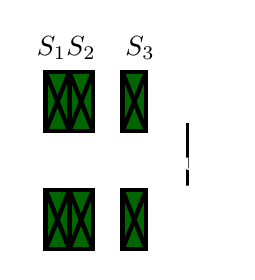
\begin{tikzpicture}[scale=0.75]
                %Gun drawings
                \draw[fill=orange, very thick, rounded corners =0.1cm] (\gunleft,0.5)rectangle (\gunright,1.5) node[pos=.5, white] {\textbf{Gun}} ;

                %S1
                \node[] at (-1.3,2.9) {$S_1$};
                \draw[ultra thick, fill=black!60!green] (-1.4,-0.5)rectangle  (-1.0,0.5) node[pos=.5, white] {} ;
                \draw[black, ultra thick] (-1.4,-0.5) -- (-1.0,0.5);
                \draw[black, ultra thick] (-1.4,0.5) -- (-1.0,-0.5);
                \draw[ultra thick, fill=black!60!green] (-1.4,1.5)rectangle  (-1.0,2.5) node[pos=.5, white] {} ;
                \draw[black, ultra thick] (-1.4,1.5) -- (-1.0,2.5);
                \draw[black, ultra thick] (-1.4,2.5) -- (-1.0,1.5);
                %S2
                \node[] at (-0.8,2.9) {$S_2$};
                \draw[ultra thick, fill=black!60!green] (-1.0,-0.5)rectangle  (-0.6,0.5) node[pos=.5, white] {} ;
                \draw[black, ultra thick] (-1.0,-0.5) -- (-0.6,0.5);
                \draw[black, ultra thick] (-1.0,0.5) -- (-0.6,-0.5);
                \draw[ultra thick, fill=black!60!green] (-1.0,1.5)rectangle  (-0.6,2.5) node[pos=.5, white] {} ;
                \draw[black, ultra thick] (-1.0,1.5) -- (-0.6,2.5);
                \draw[black, ultra thick] (-1.0,2.5) -- (-0.6,1.5);

                %S3
                \node[] at (0.2,2.9) {$S_3$};
                \draw[ultra thick, fill=black!60!green] (-0.1,-0.5) rectangle  (0.3,0.5) node[pos=.5, white] {};
                \draw[black, ultra thick] (-0.1,-0.5) -- (0.3,0.5);
                \draw[black, ultra thick] (-0.1,0.5) -- (0.3,-0.5);
                \draw[ultra thick, fill=black!60!green] (-0.1,1.5) rectangle  (0.3,2.5) node[pos=.5, white] {};
                \draw[black, ultra thick] (-0.1,1.5) -- (0.3,2.5);
                \draw[black, ultra thick] (-0.1,2.5) -- (0.3,1.5);
\end{tikzpicture}
\end{center}
\end{minipage} \hfill
\begin{minipage}{0.65\textwidth}
\begin{table}\centering
	\begin{tabular}{l c c}
		\toprule 
		\textbf{Parameter} & \textbf{Value} \\
		\midrule
		Charge  		& 1 nC \\
		$S_3$ 			&  -0.389 T \\
		$S_1$ and $S_2$ & -0.12 T \\
		Laser Radius 	& 0.75 mm \\
		Laser FWHM 		& 20 ps \\
		Laser Rise/Fall Time & 6 ps \\
		Gun Gradient 	& 60 MV/m \\
		Phase 			& Max Energy \\
		Kinetic Energy on Cathode & 0.55 eV \\
		\bottomrule
	\end{tabular}
\end{table}
\end{minipage}
\end{frame}


\begin{frame}
  \frametitle{Benchmark Results}
  \Wider[4em]{
  All codes matched within $5\%$. \\
  Well below measurement thresholds at AWA.\\  
  \vskip12pt
  \includegraphics[width=0.49\linewidth]{wikitestNoMinStep}\hfill \includegraphics[width=0.49\linewidth]{wikitest5mNoMinStep}
}
\end{frame}

%--------------------------------------------------------------------------------------------
\section{Linac Optimization}

\begin{frame}
    \frametitle{Linac Optimization: Code Used}
    \begin{itemize}
    	\setlength\itemsep{2em}
        \item Used python library NLopt: \url{http://ab-initio.mit.edu/wiki/index.php/Main_Page}
        
        \item Code summary can be found at: \url{http://www.mcs.anl.gov/~jlarson/AWA}
        
        \item Complete repo at: \url{git@xgitlab.cels.anl.gov:jmlarson/emittance_minimization.git}
    \end{itemize}	
\end{frame}

\begin{frame}
	\frametitle{Optimization using scalarization (Linac only)}
	\Wider[4em]{
	  \begin{minipage}{0.6\textwidth}
	  \begin{itemize}
	  	\item{Determine what emittance and bunch length we can expect from the linac}
	  	\begin{itemize}
		  	\item{Understand beam at entrance of quads}
	  		\item After $L_6$: $z_1=12.51$ m
	  	\end{itemize}
	  	\item{Used algorithm BOBYQA from NLopt}
	  	\item{Varied 10 parameters:}
	  \end{itemize}
	  \end{minipage}%
	  \begin{minipage}{0.4\textwidth}
		\def \gunleft {-1.0}
		\def \gunright {0.3}
		\def \loneright {1.0}
		\def \ltworight {2.0}
		\def \lthreeright {3.0}
		\def \lfourright {4.0}
		\def \lfiveright {5.0}
		\def \lsixright {6.0}
		\centering
		\begin{center}
		\begin{tikzpicture}[scale=0.55]%,use optics
		%Gun drawings
		\draw[fill=orange, very thick, rounded corners =0.1cm] (\gunleft-0.2,0.5)rectangle (\gunright,1.5) node[pos=.5, white] {\textbf{Gun}} ;
		
		%S1
		\node[] at (-1.5,2.9) {$S_1$};
		\draw[ultra thick, fill=black!60!green] (-1.4,-0.5)rectangle  (-1.0,0.5) node[pos=.5, white] {} ;
		\draw[black, ultra thick] (-1.4,-0.5) -- (-1.0,0.5);
		\draw[black, ultra thick] (-1.4,0.5) -- (-1.0,-0.5);
		\draw[ultra thick, fill=black!60!green] (-1.4,1.5)rectangle  (-1.0,2.5) node[pos=.5, white] {} ;
		\draw[black, ultra thick] (-1.4,1.5) -- (-1.0,2.5);
		\draw[black, ultra thick] (-1.4,2.5) -- (-1.0,1.5);
		%S2
		\node[] at (-0.8,2.9) {$S_2$};
		\draw[ultra thick, fill=black!60!green] (-1.0,-0.5)rectangle  (-0.6,0.5) node[pos=.5, white] {} ;
		\draw[black, ultra thick] (-1.0,-0.5) -- (-0.6,0.5);
		\draw[black, ultra thick] (-1.0,0.5) -- (-0.6,-0.5);
		\draw[ultra thick, fill=black!60!green] (-1.0,1.5)rectangle  (-0.6,2.5) node[pos=.5, white] {} ;
		\draw[black, ultra thick] (-1.0,1.5) -- (-0.6,2.5);
		\draw[black, ultra thick] (-1.0,2.5) -- (-0.6,1.5);
		
		%S3
		\node[] at (0.2,2.9) {$S_3$};
		\draw[ultra thick, fill=black!60!green] (-0.1,-0.5) rectangle  (0.3,0.5) node[pos=.5, white] {};
		\draw[black, ultra thick] (-0.1,-0.5) -- (0.3,0.5);
		\draw[black, ultra thick] (-0.1,0.5) -- (0.3,-0.5);
		\draw[ultra thick, fill=black!60!green] (-0.1,1.5) rectangle  (0.3,2.5) node[pos=.5, white] {};
		\draw[black, ultra thick] (-0.1,1.5) -- (0.3,2.5);
		\draw[black, ultra thick] (-0.1,2.5) -- (0.3,1.5);
		%Linac drawings 
		\draw[fill=blue, ultra thick, rounded corners =0.1cm] (\loneright,0)rectangle  ({\loneright+0.84},2) node[pos=.5, white] {$L_1$} ;
		\draw[fill=blue, ultra thick, rounded corners =0.1cm] (\ltworight,0)rectangle  ({\ltworight+0.84},2) node[pos=.5, white] {$L_2$};
		\draw[fill=blue, ultra thick, rounded corners =0.1cm] (\lthreeright,0)rectangle ({\lthreeright+0.84},2) node[pos=.5, white] {$L_3$};
		\draw[fill=blue, ultra thick, rounded corners =0.1cm] (\lfourright,0)rectangle ({\lfourright+0.84},2) node[pos=.5, white] {$L_4$};
		\draw[fill=blue, ultra thick, rounded corners =0.1cm] (\lfiveright,0)rectangle ({\lfiveright+0.84},2) node[pos=.5, white] {$L_5$};
		\draw[fill=blue, ultra thick, rounded corners =0.1cm] (\lsixright,0)rectangle ({\lsixright+0.84},2) node[pos=.5, white] {$L_6$};
		\end{tikzpicture}
	\end{center}
	\end{minipage}%
\begin{center}
\setcounter{mpfootnote}{\value{footnote}}%
\renewcommand{\thempfootnote}{\arabic{mpfootnote}}%	
\begin{tabular}{ l *{3}{c}}
	%\toprule
	\textbf{Variable} & \textbf{Range} & \textbf{Unit} \\
	\midrule
	Solenoid Strength & $ 0 \le S_3 \le 440$  & amps \\
	Phase of Gun & $-60 \le \phi_g \le 60$  & degrees \\
	Laser Radius  & $0.1 \le R \le 30$  & mm \\
	Laser FWHM  & $2 \le T \le $10  & ps \\
	Cavity Phase & $-20 \le \phi_L \le 20$\footnote[1]{$\phi_L=[\phi_{L_1},\ldots,\phi_{L_6}]$} & degrees
	%\bottomrule    
\end{tabular}
\end{center}
}
\end{frame}

\begin{frame}
	\frametitle{Linac Optimization}
	 \begin{itemize}
		  	\item{1,000 point sample was done}
		  	\item{132 simulations completed w/o error}
		  	\item{Scaled and shifted raw values to remove unit dependence}
	 \end{itemize}
	 \begin{align*}
	 \bar{\epsilon}_x (v,z_1) = \frac{ \epsilon_x (v,z_1) - \epsilon_{\min} } { \epsilon_{\max} - \epsilon_{\min} }
	 \end{align*}
	 
	 \begin{itemize}
	  	\item{Used 11 weights from 0-1}
	  	\item{Solved 11 optimization problems $f(v,w)$ using BOBYQA}
	 \end{itemize}
	 \begin{gather*}
	 w\in\left\{ 0, \,0.1, \,0.2, \ldots, 1 \right\}\\ \\
	 f(v,w) = w \,\bar{\epsilon}_x(v,z_1) + (1-w)\, \bar{\sigma}_z(v,z_1)
	 \end{gather*}
	

\end{frame}

\begin{frame}
	\frametitle{BOBYQA Results}
	Progress during each BOBYQA run
	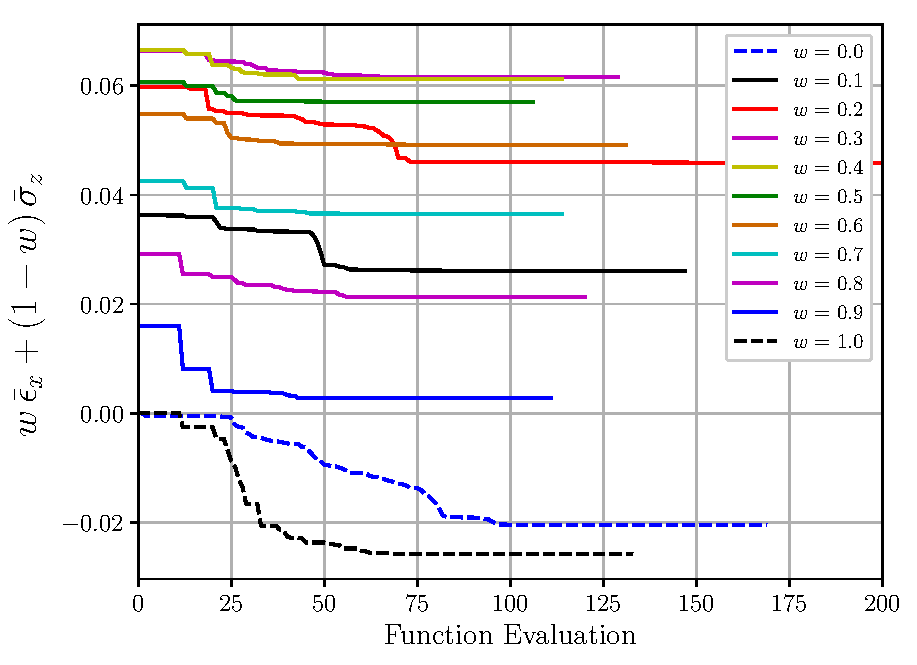
\includegraphics[width=0.9\textwidth]{THPAB155f2}
\end{frame}

\begin{frame}
	\frametitle{Approximate Pareto Front}
	\centering
	Trade off between emittance and bunch length
	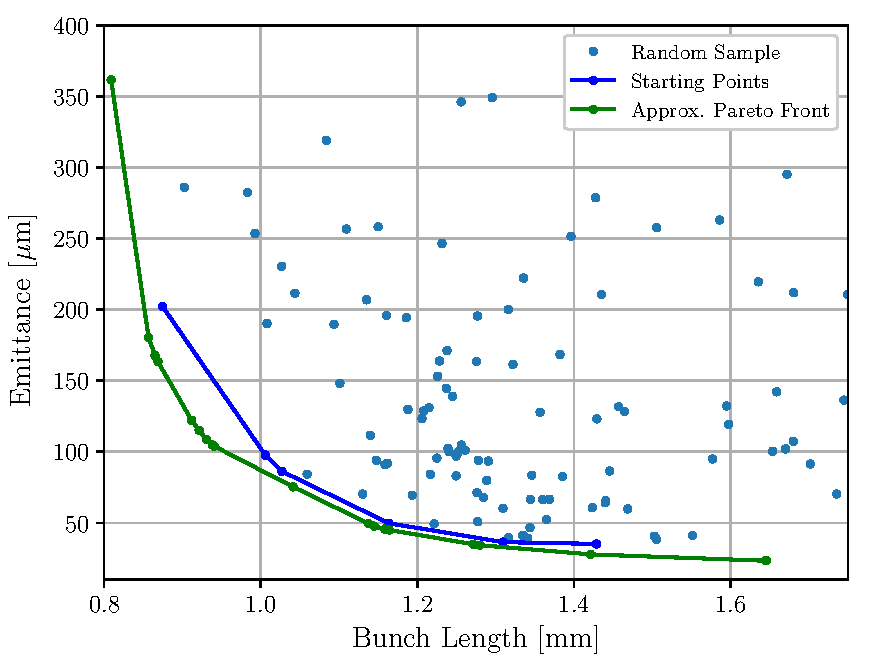
\includegraphics[width=0.85\textwidth]{THPAB155f1}
	\begin{itemize}
		\item In total, 2,492 simulations made this plot.
	\end{itemize}
\end{frame}

\section{Future Work}

\begin{frame}
	\frametitle{Beam line under design}
	\Wider[4em]{
		\def \gunleft {-1.0}
		\def \gunright {0.3}
		\def \loneright {1.0}
		\def \ltworight {2.0}
		\def \lthreeright {3.0}
		\def \lfourright {4.0}
		\def \lfiveright {5.0}
		\def \lsixright {6.0}
		\def \quadone {7.5}
		\centering
		\begin{center}
			\begin{tikzpicture}[scale=0.6]%,use optics
			%Gun drawings
			\draw[fill=orange, very thick, rounded corners =0.1cm] (\gunleft,0.5)rectangle (\gunright,1.5) node[pos=.5, white] {\textbf{Gun}} ;
			
			%S1
			\node[] at (-1.3,2.9) {$S_1$};
			\draw[ultra thick, fill=black!60!green] (-1.4,-0.5)rectangle  (-1.0,0.5) node[pos=.5, white] {} ;
			\draw[black, ultra thick] (-1.4,-0.5) -- (-1.0,0.5);
			\draw[black, ultra thick] (-1.4,0.5) -- (-1.0,-0.5);
			\draw[ultra thick, fill=black!60!green] (-1.4,1.5)rectangle  (-1.0,2.5) node[pos=.5, white] {} ;
			\draw[black, ultra thick] (-1.4,1.5) -- (-1.0,2.5);
			\draw[black, ultra thick] (-1.4,2.5) -- (-1.0,1.5);
			%S2
			\node[] at (-0.8,2.9) {$S_2$};
			\draw[ultra thick, fill=black!60!green] (-1.0,-0.5)rectangle  (-0.6,0.5) node[pos=.5, white] {} ;
			\draw[black, ultra thick] (-1.0,-0.5) -- (-0.6,0.5);
			\draw[black, ultra thick] (-1.0,0.5) -- (-0.6,-0.5);
			\draw[ultra thick, fill=black!60!green] (-1.0,1.5)rectangle  (-0.6,2.5) node[pos=.5, white] {} ;
			\draw[black, ultra thick] (-1.0,1.5) -- (-0.6,2.5);
			\draw[black, ultra thick] (-1.0,2.5) -- (-0.6,1.5);
			
			%S3
			\node[] at (0.2,2.9) {$S_3$};
			\draw[ultra thick, fill=black!60!green] (-0.1,-0.5) rectangle  (0.3,0.5) node[pos=.5, white] {};
			\draw[black, ultra thick] (-0.1,-0.5) -- (0.3,0.5);
			\draw[black, ultra thick] (-0.1,0.5) -- (0.3,-0.5);
			\draw[ultra thick, fill=black!60!green] (-0.1,1.5) rectangle  (0.3,2.5) node[pos=.5, white] {};
			\draw[black, ultra thick] (-0.1,1.5) -- (0.3,2.5);
			\draw[black, ultra thick] (-0.1,2.5) -- (0.3,1.5);
			%Linac drawings 
			\draw[fill=blue, ultra thick, rounded corners =0.1cm] (\loneright,0)rectangle  ({\loneright+0.84},2) node[pos=.5, white] {$L_1$} ;
			\draw[fill=blue, ultra thick, rounded corners =0.1cm] (\ltworight,0)rectangle  ({\ltworight+0.84},2) node[pos=.5, white] {$L_2$};
			\draw[fill=blue, ultra thick, rounded corners =0.1cm] (\lthreeright,0)rectangle ({\lthreeright+0.84},2) node[pos=.5, white] {$L_3$};
			\draw[fill=blue, ultra thick, rounded corners =0.1cm] (\lfourright,0)rectangle ({\lfourright+0.84},2) node[pos=.5, white] {$L_4$};
			\draw[fill=blue, ultra thick, rounded corners =0.1cm] (\lfiveright,0)rectangle ({\lfiveright+0.84},2) node[pos=.5, white] {$L_5$};
			\draw[fill=blue, ultra thick, rounded corners =0.1cm] (\lsixright,0)rectangle ({\lsixright+0.84},2) node[pos=.5, white] {$L_6$};
			
			%current optimization point
			%\node[draw, fill=yellow, star, star points=5, star point ratio=0.6, minimum size=0.1cm]
			%at (12.5,1.0) {$z_1$};
			
			
			%Quad drawings
			\draw[fill=black!60!green] (\quadone, 1.0) ellipse (0.2cm and 0.9cm);
			\draw[fill=black!60!green] (\quadone+0.5, 1.0) ellipse (0.2cm and 0.9cm);
			\draw[fill=black!60!green] (\quadone+1.0, 1.0) ellipse (0.2cm and 0.9cm);
			\draw[fill=black!60!green] (\quadone+1.5, 1.0) ellipse (0.2cm and 0.9cm);
			
			%Line between kicker and septum
			\draw[very thick] (\lsixright+5.3,1.0) -- (12.5,0.7);
			
			%Kicker 
			\draw[fill=orange, ultra thick, rounded corners =0.1cm] (\lsixright+3.5,0.5)rectangle ({\lsixright+0.84+4.6},1.5) node[pos=.5, white] {$Kicker$};
			
			%Septum
			\node[] at (12.7,1.5) {Septum};
			\draw[fill=black!60!green, ultra thick, rounded corners =0.1cm] (12.2,0.9)rectangle ({13.2},-0.1) node[pos=.5, white] {};
			%\draw[latex-latex] (\gunleft,-5.0) -- (14,-5.0) ;
			%\foreach \x in  {0.3, 1.0, 3.5, 5.0, 7.0, 8.5, 10, 12.5} %tick marks
			%\draw[shift={(\x,-5.0)},color=black] (0pt,3pt) -- (0pt,-3pt);
			%\foreach \x in {0.3, 1.0, 3.5, 5.0, 7.0, 8.5, 10, 12.5}
			%\draw[shift={(\x,-5.2)},color=black] (0pt,0pt) node[below] {$\x$};
			
			%Line between kicker and septum
			\draw[very thick] (13.25,0.2) -- (14.5,-0.5);
			
			%Dipole
			\node[] at (15,-1.7) {Dipole};
			\draw[fill=black!60!green, ultra thick, rounded corners =0.1cm] (14.5,0.0)rectangle ({15.6},-1.0) node[pos=.5, white] {};
			
			%Line between septum and dipole
			\draw[very thick] (15.6,-0.5) -- (16.5,-0.5);
			\end{tikzpicture}
		\end{center}

	}
	
	Optimization Parameters:
	\begin{itemize}
		\item Four quads 
		\item Distance between quads and septum
		\item Distance between kicker and septum
		\item Distance between septum and dipole
		\item Plus, 10 variables in gun and linac 
	\end{itemize}
	
\end{frame}


\begin{frame}
	\huge Thanks for your time!!\\ 
	\vskip12pt
	\large and special thanks to Andreas and Christof for always answering my OPAL-t questions by email. 
	
\end{frame}

\begin{frame}
	\frametitle{Backup: Optimized Gun Results}
	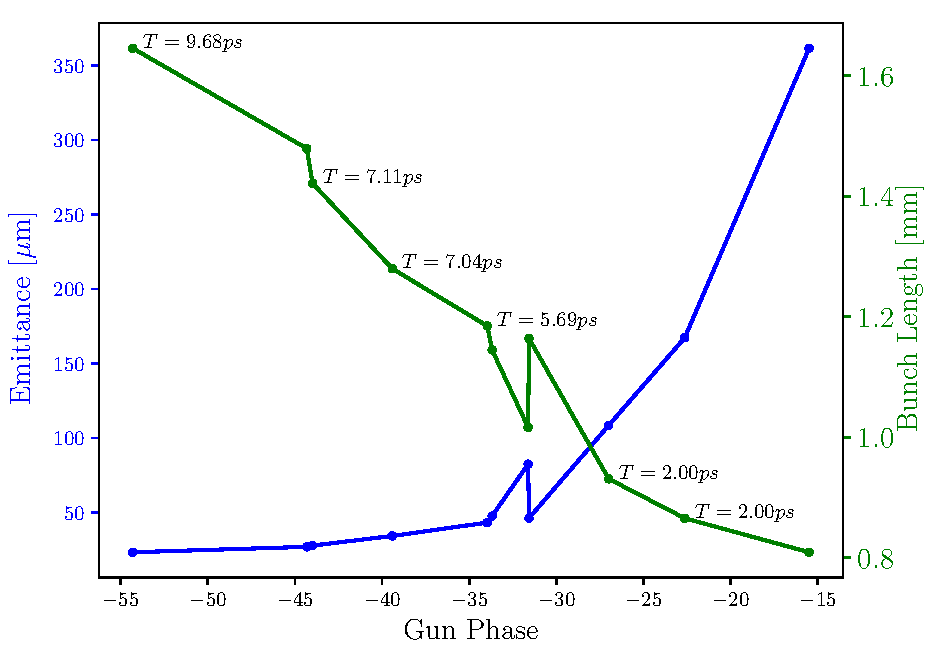
\includegraphics[width=1.0\textwidth]{THPAB155f3}
\end{frame}

\iffalse

\begin{frame}
	\begin{minipage}{0.5\textwidth}
		
	\end{minipage}%\hspace{0.2cm}
	\begin{minipage}{0.5\textwidth}
		\begin{center}
			
		\end{center}
	\end{minipage}
\end{frame}
\fi
\end{document}









